\documentclass[14pt,pscyr,titlepage]{hedreport}
\usepackage[russian]{babel}
\usepackage[utf8]{inputenc}
\usepackage[nuclear]{hedphysics}
\usepackage{hedmaths}
\usepackage{graphicx}
\usepackage{wrapfig}
\usepackage{hyperref}
\usepackage{setspace}

\graphicspath{{images//}}

\student[m]{студент группы Ф-469\\Голубев А.В.}
\teacher[m]{старший преподаватель\\Аршинов А.В.}
\faculty{Факультет электроники и вычислительной техники}
\department{<<Экспериментальная Физика>>}
\subject{методам и средствам измерительных систем}
\topic{Методы регистрации радиактивного излучения}
\type{Реферат}

\begin{document}
	\maketitle
	\tableofcontents
	\onehalfspacing
	\section{Введение}
		Для рассмотрения методов регистрации радиактивного излучения нужно 
		сначала определиться что же такое радиоактивность и ввести некоторые 
		термины. 

		Ядро может находиться в различных состояниях с дискретными 
		значениями энергии. Состояние с наименьшей энергией называется 
		основным, соответственно, значение энергии в этом состоянии называется 
		основным уровнем энергии ядра. Другие состояния называются 
		возбужденными. Переход ядра из возбужденного состояния в основное 
		сопровождается излучением \( \gamma \)-кванта. Явление испускания 
		атомами невидимых проникающих излучений, открытое в 1896 году. 
		французским физиком Анри Беккерелем, назвали радиоактивностью.

		Не всякое атомное ядро, состоящее из протонов и нейтронов, 
		удерживаемых ядерными силами притяжения, может существовать 
		неограниченно долго: эти силы обладают свойством насыщения, поэтому 
		дефицит или избыток нейтронов делают ядра атомов неустойчивыми.

		Радиоактивность -- это свойство атомных ядер спонтанно изменять свой 
		состав: заряд ядра \( Z \) и число нуклонов \( A \), путем испускания 
		элементарных частиц, \( \gamma \)-квантов или ядерных фрагментов.

		Альфа-распадом называется самопроизвольный распад атомного ядра на 
		\( \alpha \)-частицу (ядро атома гелия \( \nucleus{4}{2}{He} \)) и 
		ядро-продукт. Начальная кинетическая энергия всех \( \alpha \)-частиц, 
		испускаемых ядрами одного изотопа, одинакова или 2-3-х разных 
		значений, т.к. довольно часто часть энергии \( \alpha \)-распада 
		может пойти на возбуждение ядра-продукта, которое спустя короткое 
		время после вылета \( \alpha \)-частицы испускает один или несколько 
		\( \gamma \)-квантов и переходит в основное состояние.

		В основе бета-распада лежит способность протонов и нейтронов к 
		взаимным превращениям. При самопроизвольном превращении нейтрона в 
		протон испускается электрон и антинейтрино; протон же испускает 
		позитрон и нейтрино, превращаясь в нейтрон. Энергетический спектр 
		\( \beta \)-частиц сплошной, начиная от нуля и до некоторого 
		максимального значения, называемого максимальной энергией 
		\( \beta \)-спектра, т.к. часть энергии \( \beta \)-распада уносят 
		нейтрино (антинейтрино).

		Как и \( \alpha \)-распад, он может сопровождаться 
		\( \gamma \)-излучением. К бета-распаду относится и \( К \)-захват, 
		когда ядро захватывает с ближайшей оболочки К один электрон и протон 
		превращается в нейтрон.

	\section{Взаимодействие ядерных излучений с веществом}
		При движении заряженной частицы в веществе происходит поглощение ее 
		энергии за счет взаимодействия с электронными оболочками и ядрами 
		атомов. При упругих столкновениях происходит рассеяние потока 
		излучения, при неупругих столкновениях с электроном оболочки последний 
		получает дополнительную энергию и переходит на одну из более удаленных 
		от ядра орбит или совсем покидает атом. В первом случае происходит 
		возбуждение, во втором -- ионизация атома. Потери энергии на 
		возбуждение и ионизацию атомов среды называются ионизационными.

		Если энергии частицы достаточно для выбивания электрона из внутренних 
		слоев оболочек атома, то возникает характеристическое рентгеновское 
		излучение с линейчатым спектром. 

		При прохождении вблизи ядра быстрая заряженная частица испытывает 
		торможение в его электрическом поле, сопровождаемое испусканием квантов 
		тормозного рентгеновского излучения. Потери энергии на излучение 
		называются радиационными. 

		При одинаковой начальной энергии тяжелые частицы (\( \alpha \), 
		протоны) обладают меньшими скоростями, чем легкие. Медленно движущиеся 
		частицы взаимодействуют с атомами более эффективно и быстро 
		растрачивают имеющийся у них запас энергии на ионизацию атомов 
		вещества, радиационные потери при этом малы.

		Гамма-кванты не обладают электрическим зарядом и поэтому свободно 
		проходят сквозь большинство встречающихся на их пути атомов, но и 
		они испытывают упругие и неупругие столкновения с электронами атомов, 
		рассеиваясь или тратя свою энергию на выбивание электронов из 
		атомов. Эти вторичные электроны и производят ионизацию и возбуждение 
		атомов среды.

        Таким образом, конечными результатами взаимодействия с веществом 
        любого вида ядерного излучения являются ионизация и возбуждение атомов 
        среды, поэтому ядерные излучения и называют ионизирующими излучениями.

		Наибольшей проникающей способностью обладает гамма-излучение, а 
		наибольшей ионизационной способностью -- альфа-частицы, бета-излучение 
		занимает промежуточное положение по обоим этим свойствам. В немалой 
		степени эти свойства зависят от начальной энергии излучения и 
		плотности среды, в плотной среде бета-излучение может вызвать 
		значительное тормозное излучение, что необходимо учитывать при 
		расчете защиты.

	\section{Методы регистрации излучений}
		Радиоактивное излучение не может быть обнаружено непосредственно ни 
		одним из наших органов чувств. Для обнаружения и оценки воздействия 
		излучений на человеческий организм  пользуются различными методами. 
		Разработка методов детектирования и измерения радиоактивных излучений 
		является предметом специальной области технической физики -- 
		дозиметрии. Приборы, применяемые для этих целей, называются 
		радиометрическими и дозиметрическими.

		Радиометрические приборы служат для измерения активности радиоактивных 
		веществ, плотности потока ионизирующего излучения; удельной и объемной 
		активности газов, жидкостей, аэрозолей; удельной поверхностной активности.

		Дозиметрические приборы служат для измерения экспозиционной дозы 
		рентгеновского и гамма-излучения; поглощенной дозы излучений; мощности 
		поглощенной дозы; интенсивности ионизирующих излучений. 

		Все методы обнаружения излучений основаны на взаимодействии последних с 
		веществом и различаются как по характеру учитываемого взаимодействия, 
		так и по способам измерения.

		В основу всех дозиметрических и радиометрических приборов положен 
		один из следующих методов регистрации ионизирующих излучений:
		\begin{enumerate}\itemsep-2pt
			\item ионизационный,
			\item люминесцентный (сцинтилляционный),
			\item фотографический,
			\item калориметрический,
			\item химический.
		\end{enumerate}

	\subsection{Ионизационный метод} 
		Под действием любого ионизирующего излучения в веществе, газе из 
		нейтральных атомов или молекул образуются ионы -- частицы, несущие 
		положительные или отрицательные электрические заряды. В обычных 
		условиях образовавшиеся ионы существуют недолго, они рекомбинируют, 
		т.е. вновь соединяются в нейтральные атомы или молекулы. Применение 
		ионизационных камер основано на использовании способности газов под 
		воздействием радиоактивных излучений становиться проводниками 
		электрического тока. В электрическом поле подвижные ионы газа довольно 
		быстро перемещаются к соответствующим электродам, вследствие чего 
		рекомбинация незначительна. Имеется три вида ионизационных газовых 
		детекторов излучения.

		\emph{1. Ионизационная камера. }

		Принцип действия ионизационной камеры основан на ионизации атомов 
		газа, заполняющего ка-меру, ионизирующими частицами или квантами 
		излучения. В камере расположены два металлических электрода, к 
		которым приложена разность потенциалов, создающая электрическое поле 
		в пространстве между электродами. Ионы, образованные в камере 
		ионизирующим излучением -- \( \beta \)-частицами или квантами 
		электромагнитного излучения, - двигаются в электрическом поле к 
		электродам, полярность которых противоположна знаку заряда ионов. 
		В камере возникает ток, величина которого пропорциональна числу ионов, 
		создаваемых излучением в камере и, следовательно, пропорциональна 
		интенсивности излучения.

		Основное дозиметрическое соотношение для ионизационной камеры имеет 
		вид:
		\[
			X = \frac{W}{eV\rho}i_\text{нас}
		\]
		где: \( X \) -- мощность экспозиционной дозы, \( W \) -- средняя 
		энергия образования одной пары ионов в воздухе, 34 эВ, \( e \) -- 
		заряд иона, \( V \) -- ионизационный объём газа (камеры), 
		\( \rho \) -- плотность газа, \( i_\text{нас} \) -- ток насыщения.

		Если приложенную к цепи разность потенциалов постепенно увеличивать 
		при постоянной интенсивности излучения, то оказывается, что ток в 
		цепи вначале увеличивается пропорционально приложенной разности 
		потенциалов, затем он становится постоянным по величине, несмотря на 
		увеличение разности потенциалов, т.е. достигает значения насыщения.

		На рисунке показана зависимость величины импульса от приложенного к 
		электродам газовой ка-меры напряжения. Область 1 соответствует работе 
		ионизационных камер. Ионизационные камеры работают при небольших 
		напряжениях 100-200 В.

		\begin{figure}[h!]
			\center
			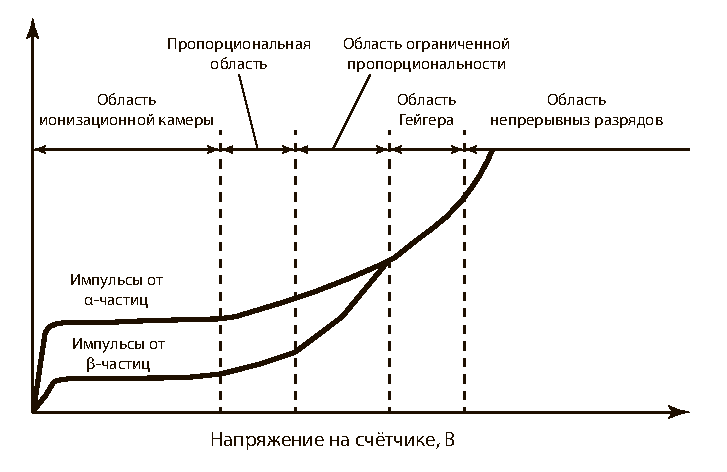
\includegraphics[width=.8\textwidth]{counter_graph} \\
			\caption{Зависимость величины импульса от приложенного к электродам 
				газовой камеры напряжения}
			\label{img:graph}
		\end{figure}

		Основными недостатками ионизационных камер являются малая величина 
		получаемого сигнала и низкая эффективность регистрации квантового 
		излучения.

		Если на электродах ионизационной камеры поднять напряжение до 
		300-500 В, то электроны и ионы, создаваемые ионизирующим излучением в 
		объеме камеры, ускоряясь в электрическом поле, сами становятся 
		ионизирующими агентами, образуя вторичные ионы. Этот процесс 
		называется газовым усилением. Коэффициент газового усиления может 
		изменяться от \( 10 \) до \( 10^6 \).

		\emph{2. Пропорциональные счетчики. }

		Ионизационная камера, работающая в режиме газового усиления, 
		называется пропорциональным счетчиком (область 2 на \ref{img:graph}). 
		В пропорциональных счетчиках используется для усиления ионизации 
		несамостоятельный разряд, при котором электроны, созданные 
		ионизирующей частицей, двигаясь в электрическом поле, набирают 
		энергии, достаточной для ионизации ударом. Разряд в них прекращается 
		сразу же, как только образовавшиеся ионы достигнут соответствующих 
		электродов. Пропорциональные счетчики в отличие от ионизационных 
		камер работают в импульсном режиме и их применяют для измерения 
		энергии частиц и регистрации излучения определенного типа в 
		присутствии другого излучения.

		\emph{3. Газоразрядные счетчики (Гейгера-Мюллера). }

		Пропорциональные счетчики, работающие в режиме газового разряда, 
		называются газоразрядными (см. \ref{img:graph} область 4). Разность 
		потенциалов, приложенная  к электродам, настолько велика 
		(1200-1500 В), что в камере может происходить самостоятельный разряд, 
		поэтому счетчик отмечает вспышкой самостоятельного разряда практически 
		каждую из частиц, создающих ионизацию в его чувствительном объеме. Для 
		возможности регистрации следующих частиц разряд в счетчике должен 
		быть погашен каким-либо образом. Для гашения разряда в атмосферу 
		счетчика из одно-атомного газа (неон, аргон и  др.) вводят небольшое 
		количество многоатомного газа (пары спирта, этилен, изопентан, хлор 
		или бром), вследствие чего самостоятельный разряд прекращается 
		примерно через \( 10^{-7} \) секунд с момента возникновения. Такие 
		счетчики называются самогасящимися. Для гашения разряда в 
		несамогасящемся счетчике в его цепь последовательно включается 
		высокоомный резистор, понижающий напряжение на аноде. 

		Величина выходного импульса не зависит от типа и энергии ионизирующей 
		частицы. Газоразрядные счетчики имеют небольшую эффективность 
		регистрации квантового излучения : 1-2\% при энергии квантов 1 МэВ.

		Любой счетчик характеризует эффективность регистрации:
		\[
			\eta = \frac{N_\text{зарег.}}{N_\text{падающ.}}\cdot 100\%
		\]
		где \( N_\text{зарег.} \) -- число зарегистрированных частиц, 
		\( N_\text{падающ.} \) -- число частиц, попавших в объём счётчика.

		Основное достоинство ионизационного метода -- непосредственное 
		преобразование энергии ионизирующего излучения в электрический сигнал, 
		возможность усиления сигнала, простота устройства детектора. 
		Некоторые неудобства в том, что требуется дополнительная электронная 
		аппаратура, стабилизаторы высокого напряжения, регистрирующие схемы с 
		широким диапазоном чувствительности и пр.

	\subsection{Фотографический метод}
		Фотографический метод дозиметрии основан на способности ионизирующих 
		излучений засвечивать защищенную от попадания видимого света 
		фотопленку. В настоящее время это метод используют для индивидуального 
		контроля экспозиционной дозы рентгеновского, гамма-, бета- и 
		нейтронного излучений, при измерении космического излучения и 
		высокоэнергетических ускорителей. Химически обработанная пленка имеет 
		прозрачные и почерневшие места, которые соответствуют незасвеченным и 
		засвеченным участкам фотоэмульсии.

		Почернение -- это мера облучения пленки, оно определяется по 
		ослаблению светового потока при прохождении через фотослой. Отношение 
		интенсивности падающего светового пучка к интенсивности прошедшего 
		через пленку называется  коэффициентом непропускания фотопленки, а 
		величина, равная логарифму коэффициента непропускания -- оптической 
		плотностью почернения:
		\[
			S = \lg\frac{I_0}{I}
		\]

		Измерение ее производится с помощью денситометра, сравнивая почернение 
		пленки в индивидуальном дозиметре с эталонной или контрольной 
		пленкой, определяют дозу, воздействовав-шую на человека. 

		Фотографический метод дозиметрии обладает следующими 
		преимуществами -- возможность массового применения для индивидуального 
		дозиметрического контроля, невосприимчивость к ударам, резкому 
		изменению температуры, документальная регистрация полученной дозы.

		К недостаткам метода относятся -- относительно небольшая 
		чувствительность к малым эквивалентным дозам, невозможность измерения 
		дозы непосредственно в момент облучения, сложность фотообработки, 
		зависимость показаний от условий фотообработки и измерений.

	\subsection{Химический метод}
		Химический метод основан на измерении числа молекул или ионов, 
		образующихся или претерпевших изменения при поглощении веществом 
		ионизирующего излучения. Число образующихся молекул или ионов, так
		называемый радиационно-химический выход пропорционален поглощенной 
		дозе излучения. Многие химические дозаторы представляют собой водные 
		растворы некоторых веществ. Появление новых молекул или ионов изменяет 
		оптическую плотность раствора, которая измеряется  спектрофотометром, 
		или меняет цвет раствора. Густота окраски при этом пропорциональна 
		дозе облучения. Определение густоты окраски может быть произведено 
		денситометром.

		Химическим методом можно измерять большие дозы излучений, но он 
		значительно уступает по чувствительности фотографическому, 
		ионизационному и сцинтилляционному. Кроме того, химические дозиметры 
		требуют значительного расхода материалов и известного времени для 
		снятия показаний.

	\subsection{Калориметрический метод}
		Тепловой, калориметрический метод дозиметрии возможен потому, что в 
		конечном итоге вся поглощенная веществом энергия переходит в тепло. 
		Количество тепла, выделяемого облучаемым веществом, пропорционально 
		произведению числа частиц на их среднюю энергию. Поэтому, измерив 
		выделившееся тепло, можно определить количество поглощенной энергии, а 
		зная средней энергии частицы -- определить число частиц.      

		Этот метод абсолютный, единственный прямой, в этом его преимущество. 
		Результаты не зависят от самопоглощения, рассеяния излучения, характера 
		взаимодействия и пр. Но чувствительность очень низка, пригоден для 
		измерения высоких активностей и мощных потоков излучения.

	\subsection{Люминесцентный метод}
		Люминесцентные методы измерения ионизирующих излучений. 
		Люминесценция -- <<холодно>> свечение вещества, возбуждаемое светом, 
		радиоактивным излучением и т.п.

		При облучении ионизирующим излучением люминофоров происходит следующее:
		\begin{itemize}\itemsep-2pt
			\item поглощение энергии излучения и переход вещества в 
				неравновесное состояние;
			\item преобразование поглощенной энергии;
			\item испускание света (или возникновение других оптических 
				эффектов) при переходе вещества в равновесное состояние, 
				что может служить мерой поглощенной дозы.
		\end{itemize}

		Процессы люминесценции, используемые в дозиметрии можно разделить 
		на четыре группы:
		\begin{itemize}\itemsep-2pt
			\item сцинтилляционные -- нестимулированные с быстрым 
				высвечиванием центров люминесценции;
			\item процессы, характеризующиеся запасенной светосуммой и 
				последующим стимулированным высвечиванием центров 
				люминесценции;
			\item процессы, приводящие к тушению нормальной люминесценции;
			\item процессы, приводящие к образованию центров окраски.
		\end{itemize}

		Последние основаны на окрашивании стекол и пластиков.

		Детекторы ионизирующего излучения, основанные на стимулировании 
		люминесценции в твердых телах и на окрашивании стекол и пластиков, 
		отличаются простотой в изготовлении, низкой стоимостью, длительным 
		сроком службы, безотказностью в работе, небольшими габаритами, широким 
		диапазоном регистрации поглощенной дозы.

		Сцинтилляционные счетчики (лат. sintillatio -- сверкание, искрение). 
		Вещества, испускающие свет под действием ионизирующего излучения, 
		называются сцинтилляторами. Сцинтилляционный счетчик представляет 
		собой комбинацию сцинтилляционного кристалла с ФЭУ 
		(фотоэлектронным умножителем) и регистрирующей электронной схемой. 
		ФЭУ позволяет преобразовать слабые световые вспышки от сцинтиллятора 
		в достаточно большие электрические импульсы. Поглощенная энергия в 
		кристалле \( E_\text{П} \) в основном расходуется на ионизацию и 
		возбуждение, в процессе которых часть энергии может переходить в 
		теплоту. Возбужденные же молекулы и атомы кристалла вновь излучают 
		энергию в виде фотонов света \( E_\text{Ф} \).

		Эффективность преобразования энергии заряженных частиц в световую 
		энергию фотонов называется конверсионной эффективностью сцинтиллятора 
		(физический световой выход) и определяется отношением:
		\[
			\eta_K = \frac{E_\text{Ф}}{E_\text{П}}
		\]

		Сцинтилляционные счетчики применяются для измерения числа заряженных 
		частиц, \( \gamma \)-фотонов, быстрых и медленных нейтронов; для 
		измерения мощности дозы \( \beta \)-, \( \gamma \)- и нейтронного 
		излучений и в некоторых случаях для исследования спектров 
		\( \gamma \)- и нейтронного излучений.

		Чувствительность сцинтилляционных счетчиков на несколько порядков выше 
		чувствительности ионизационных камер и газовых пропорциональных 
		счетчиков. Малое время высвечивания (процесса выхода световой энергии 
		из сцинтиллятора) обеспечивает ему малое мертвое время, что позволяет 
		проводить измерения с короткоживущими радионуклидами.

		На процессах с запасенной светосуммой основаны радиофотолюминесцентные 
		и термолюминесцентные детекторы. Под действием излучения в люминофоре 
		создаются центры фотолюминесценции, последующее стимулирование 
		которых вызывает видимую люминесценцию. РФЛ-дозиметры стимулируются 
		ультрафиолетовым светом, интенсивность <<холодного свечения>> 
		пропорциональна поглощенной дозе. При этом образованные центры не 
		разрушаются, некоторые типы РФЛ-дозиметров сохраняют информацию в 
		течение нескольких лет. Их недостатком является уменьшение 
		чувствительности за счет укрупнения зерна после отжига, которым 
		производится снятие предыдущих показаний.

		В ТЛД в качестве стимулятора высвечивания используется нагрев.

		Дозиметры ТЛД и РФЛ удобны в качестве индивидуальных дозиметров. 
		По чувствительности и диапазону измерения доз, длительности хранения 
		информации они значительно превосходят ионизационные и фотопленочные 
		индивидуальные дозиметры. 

	\pagebreak
	\section{Трековые детекторы}
		Трековые или следовые детекторы позволяют наблюдать визуально треки 
		проходящих частиц. К ним относится: камера Вильсона, пузырьковая 
		камера, ядерные фотоэмульсии, искровые камеры.

		Общий принцип регистрации основан на том, что ускоренные заряженные 
		частицы, попадая в рабочее вещество, ионизируют его по ходу движения. 
		В результате ионизации вещества возникают вторичные эффекты, которые 
		можно наблюдать и по ним оценивать наличие частиц, их энергию, 
		среднюю длину пробега и т.д.

	\subsection{Камера Вильсона}
		\begin{wrapfigure}[14]{l}{0.5\textwidth}
			\vspace{-2ex}
			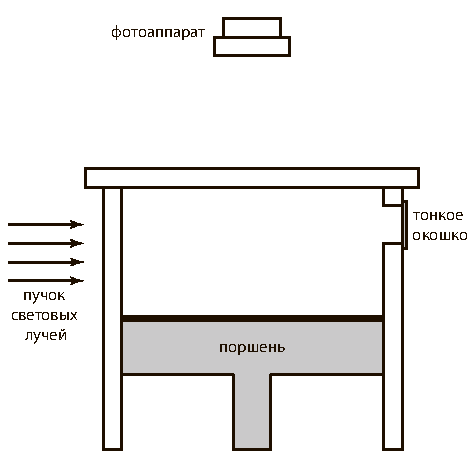
\includegraphics[width=0.5\textwidth]{wilson_cam}
			\parbox{0.5\textwidth}{\caption{Схематичное изображение}}
		\end{wrapfigure}
		В качестве рабочего вещества используется пересыщенный пар. В состав 
		пара входит вода, этиловый спирт, гелий и аргон. Камера представляет 
		собой стеклянный цилиндрический сосуд, покрытый сверху стеклом. Над 
		этим стеклом располагается фотокамера. Снизу сосуда 
		расположен подвижный поршень, над поршнем располагается сетка, 
		покрытая слоем черного влажного бархата или сукна.

		При быстром опускании поршня происходит адиабатическое расширение 
		газа, что сопровождается понижением его температуры. За счет 
		охлаждения пар становится переохлажденным. 

		Заряженные частицы, пролетая в газе, создают на своем пути цепочку 
		ионов. На этих ионах как на центрах конденсации образуются капельки 
		жидкости. Таким образом, при движении в камере частица оставляет за 
		собой трек, который хорошо виден и может быть сфотографирован. По 
		геометрии полученных треков можно определить количество частиц и 
		направления их движения. Если весь трек умещается в камере, то можно 
		установить энергию частицы, средний линейный пробег, линейную 
		плотность ионизации. При помещении камеры в постоянное магнитное 
		поле можно по радиусу кривизны траектории определить удельный заряд, 
		скорость и энергию частиц.

	\subsection{Пузырьковая камера}
		В качестве  рабочего вещества используют перегретую жидкость, 
		закипающую при резком уменьшении ее давления. В качестве рабочих 
		жидкостей применяют жидкий водород, пропан \( C_3 H_8 \), ксенон и 
		другие легко кипящие жидкости. При движении заряженных частиц 
		образуются ионы, являющиеся центрами интенсивного парообразования, 
		приводящие к появлению цепочки пузырьков. В пузырьковой камере можно 
		регистрировать частицы очень больших энергий, т.к. частицы тормозятся 
		в ней на отрезках в тысячу раз меньших, чем в камере Вильсона. 

	\subsection{Толстослойные фотоэмульсии}
		Этот метод основан на фотохимическом действии ионизирующего излучения. 
		Под действием проходящих через фотоэмульсию быстрых заряженных частиц 
		нарушается структура кристаллической решетки зерен бромистого серебра, 
		делающих их неспособных к проявлению, поэтому после проявления 
		получают цепочку черных точек, которые видны под микроскопом. Ядерные 
		эмульсии применяются в виде слоев толщиной от 0,5 до 1 мм. Это 
		позволяет исследовать траектории частиц высоких энергий. Например, 
		частица с энергией порядка 10 МэВ образует след длиной 0,1 мм и не 
		выходит за пределы слоя. 

    	Для изучения треков частиц с еще большей энергией и имеющих средний 
    	линейный пробег больше толщины одной пластины используют стопу из 
    	большого числа пластин.  Стопу пластин располагают наклонно к следу. 
    	В этом случае последовательные участки следов траектории частицы можно 
    	изучать по почернению эмульсии в пластинках стопы, следующих друг 
    	за другом. 

    \pagebreak
	\section{Счётчики и интегральные приборы}
	\subsection{Счётчик Гейгера-Мюллера}
		\begin{wrapfigure}[12]{l}{0.5\textwidth}
			\vspace{-2ex}
			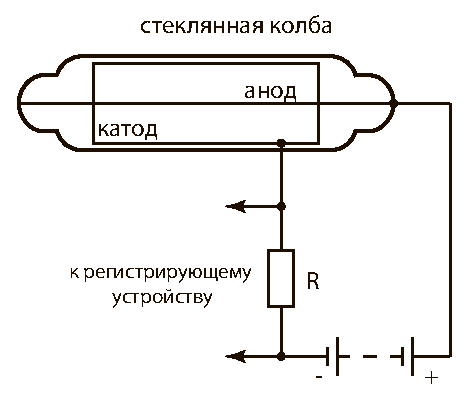
\includegraphics[width=0.5\textwidth]{geyger-myuller_counter}
			\parbox{0.5\textwidth}{\caption{Схематичное изображение}}
		\end{wrapfigure}
		Это устройство позволяет считать число частиц, попадающих в 
		устройство. Принцип его действия основан на ионизации газа под 
		действием различных видов ионизирующего излучения.

 		Счетчик представляет собой геометрически запаянную стеклянную трубку, 
 		к внутренним стенкам которой прилегает катод –- тонкий металлический 
 		цилиндр; анодом служит тонкая проволока, натянутая по центрально оси 
 		счетчика. Рабочее напряжение составляет сотни вольт. 

		Счетчик включается в регистрационную схему. На корпус подается 
		отрицательный потенциал, на нить -- положительный. Последовательно 
		счетчику включается резистор с сопротивлением  несколько мегом. С 
		резистора через разделительный конденсатор с емкостью несколько тысяч 
		микрофарад сигнал подается на вход пересчетной схемы. Внутри трубки 
		находится смесь газов под атмосферным или пониженным давлением. Газ 
		является хорошим диэлектриком и при отсутствие ионизирующих частиц, 
		тока во внешней цепи нет.  

		Если в счетчик попала хотя бы одна ионизирующая частица, то она 
		создает одну паров ионов. Положительный ион и электрон движутся в 
		поле с одинаковой напряженностью, но длина свободного пробега 
		электрона много больше длины свободного пробега положительного иона, 
		поэтому электрон является более эффективным ионизатором. Под действием 
		электрического поля  кинетическая энергия электронов возрастает и 
		становится больше энергии ионизации атомов газовой смеси, поэтому 
		при взаимодействии образовавшегося электрона с атомами  образуются 
		новые ионы и электроны. Происходит ударная ионизация газа. При ударной 
		ионизации и высокой напряженности электрического поля в газе создается 
		ионная лавина.        

		Вторичные электроны, возникающие за счет  ударной ионизации, также 
		разгоняются полем и в свою очередь ионизируют встречные атомы и 
		молекулы. В результате такой цепной реакции даже небольшое число 
		электронов, возникающее в результате внешней ионизации, резко 
		увеличивает электропроводность  газа, вследствие чего по резистору 
		течет ток и на его концах возникает импульс напряжения, который через 
		конденсатор поступает на вход пересчетного устройства.

		Высокий потенциал, который первоначально находился на аноде, 
		переключается на резистор, напряженность электрического поля внутри 
		счетчика убывает, вследствие чего уменьшается кинетическая энергия 
		электронов, что приводит прекращению режима газового усиления.

	\subsection{Сцинтилляционный счётчик}
		При попадании \( \alpha \)-частиц на флуоресцирующие вещества они 
		вызывают слабые световые вспышки -- так называемые сцинцилляции. Было 
		установлено, что каждая попавшая на такое вещество 
		\( \alpha \)-частица вызывает одну вспышку и это может быть 
		использовано для счета \( \alpha \)-частиц.

		\begin{figure}[h!]
			\center
			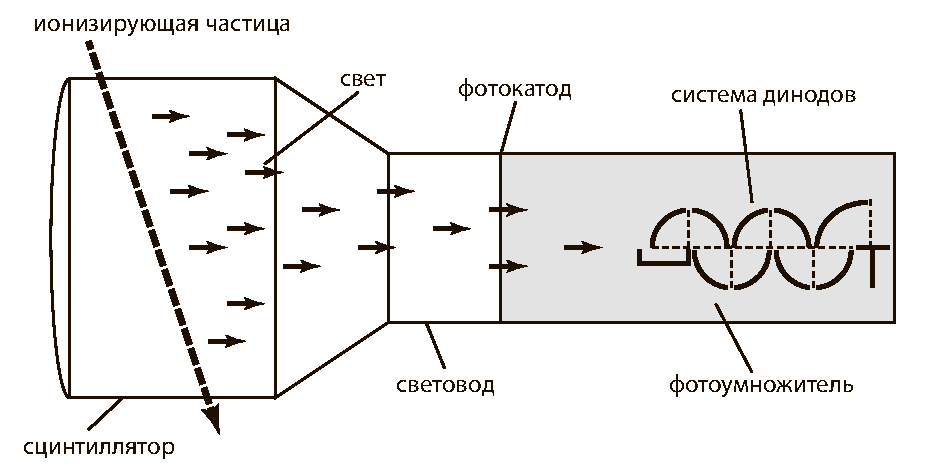
\includegraphics[width=.8\textwidth]{scintillascope} \\
			\caption{Сцинтилляционный счётчик}
			\label{img:graph}
		\end{figure}

		В конце сороковых годов были построены сцинтилляционные счетчики частиц. 
		Такой счетчик состоит из флуоресцирующего вещества. В качестве 
		люминофоров используются кристаллы: йодистый натрий или калий, 
		нафталин, антрацен и другие. Применяются также жидкие люминофоры, 
		например, раствор трифенила в ксилоле. Частицы, обладающие достаточно 
		большой энергией попадая в вещество, вызывают сцинтцилляционные 
		вспышки. Каждая вспышка действует на фотокатод электронного умножителя 
		и выбивает из него электроны. Электроны, проходя через n каскадов 
		умножителя, дают на выходе импульс тока, который затем подается на 
		вход усилителя. Усиленный электрический импульс подается на 
		регистрирующее устройство. С помощью осциллографа можно определить 
		интенсивность отдельных импульсов. Эта интенсивность пропорциональна 
		энергии отдельной сосчитанной частицы. Таким образом, определяют не 
		только число частиц, но и распределение их по энергиям. 

	\pagebreak
	\section{Приборы}
	\subsection{Дозиметр радиометр ДКС-96}
		\emph{Область применения:} службы дозиметрического контроля на объектах 
		атомной энергетики и промышленности, в том числе на судах с ядерными 
		энергетическими установками, в медицинских, научных и других 
		учреждениях, как самостоятельно, так и в составе автоматизированных 
		систем радиационного контроля.
		
		\emph{Измерение:} плотность потока альфа-излучения, плотность потока 
			бета-излучения, рентгеновское и гамма-излучение. 

		\emph{Тип детектора:} сцинтилляционный

		\begin{figure}[h!]
			\center
			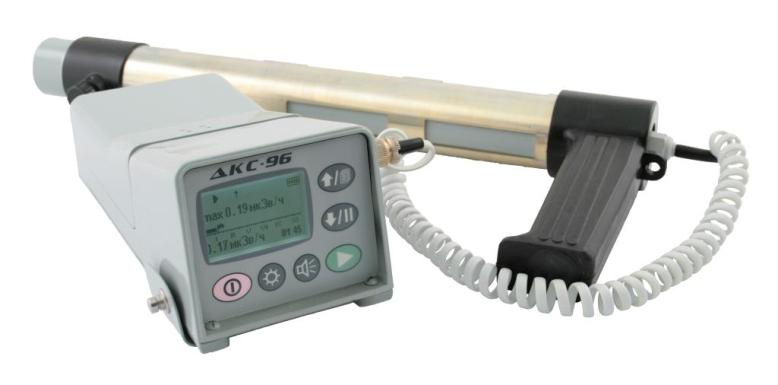
\includegraphics[width=.8\textwidth]{DKS-96} \\
			\caption{Внешний вид ДКС-96}
		\end{figure}

	\pagebreak

	\subsection{Радиометр радона РРА-01М-01}
		\emph{Область применения:} применяется на объектах сферы обороны, 
			безопасности и в промышленности для комплексного 
			санитарно-гигиенического обслуживания территорий.

		\emph{Измерение:} радон-222

		\emph{Тип детектора:} полупроводниковый

		\begin{figure}[h!]
			\center
			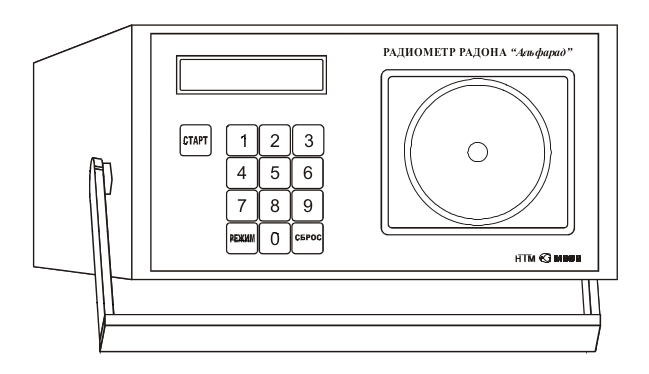
\includegraphics[width=.8\textwidth]{RRA-01M-01} \\
			\caption{Внешний вид РРА-01М-01}
		\end{figure}

	\pagebreak

	\subsection{Спектрометр СКС-99 <<Спутник>>}
		\emph{Область применения:} предназначена для спектрометрических, 
			радиометрических и дозиметрических измерений ионизирующих 
			излучений.

		\emph{Измерение:} удельная активность альфа-, бета-, гамма-излучающих 
			радионуклидов,  плотность потока нейтронного излучения, плотность 
			потока бета-частиц, мощность эквивалентной дозы гамма-излучения.

		\emph{Тип детектора:} сцинтилляционный с ФЭУ, счётчик Гейгера

		\begin{figure}[h!]
			\center
			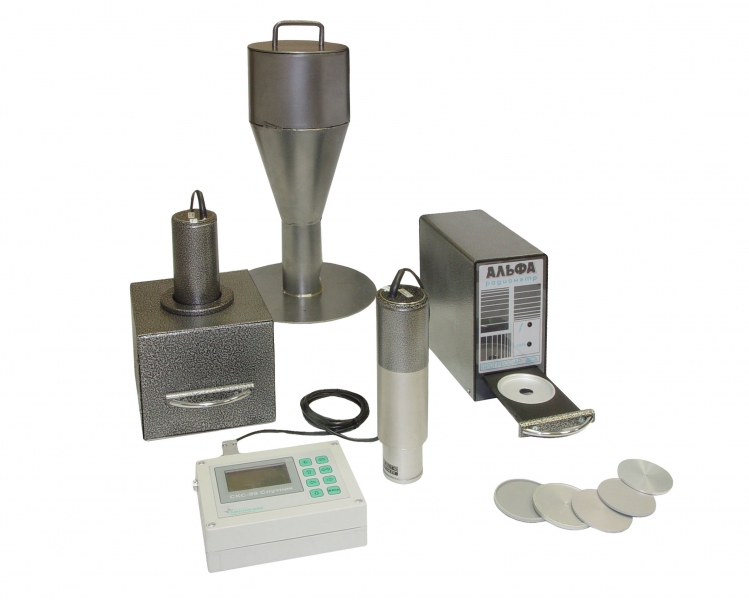
\includegraphics[width=.8\textwidth]{CKC-99} \\
			\caption{Внешний вид СКС-99 <<Спутник>>}
		\end{figure}

	\pagebreak

	\section{Список используемой литературы}
	\begin{enumerate}\itemsep-2pt
		\item Пособие для дозиметриста [Текст] : учебное пособие для 
			дозиметристов // ЗАО <<Титан-Изотоп>>, 2005
		\item Дозиметры-радиометры ДКС–96 [Электронное издание] : руководство 
			по эксплуатации / Научно-производственное предприятие 
			<<Доза>>. --- 2010. --- Режим доступа: 
        	\href{http://ntcpoisk.ru/d/350762/d/dozimetri_radiometridks96.pdf}
        		{http://ntcpoisk.ru}  
        \item Радиометр радона портативный РРА-01М-01 [Электронное издание] : 
        	руководство по эксплуатации. --- Режим доступа:
        	\href{http://www.baz-alt.ru/userfiles/files/sks.pdf}
        		{http://www.baz-alt.ru}  
        \item Установка спектрометрическая СКС-99 <<СПУТНИК>> 
			[Электронное издание]: рук-во по эксплуатации. --- Режим доступа: \\
			\href{http://www.electronpribor.ru/resources/docs/RE_PPA_01_01ispr.pdf}
				{http://www.electronpribor.ru}
	\end{enumerate}
\end{document}